\documentclass[tikz,border=15pt]{standalone}
\usepackage{tikz}
\usetikzlibrary{shapes.geometric, arrows.meta, positioning, calc}

\begin{document}
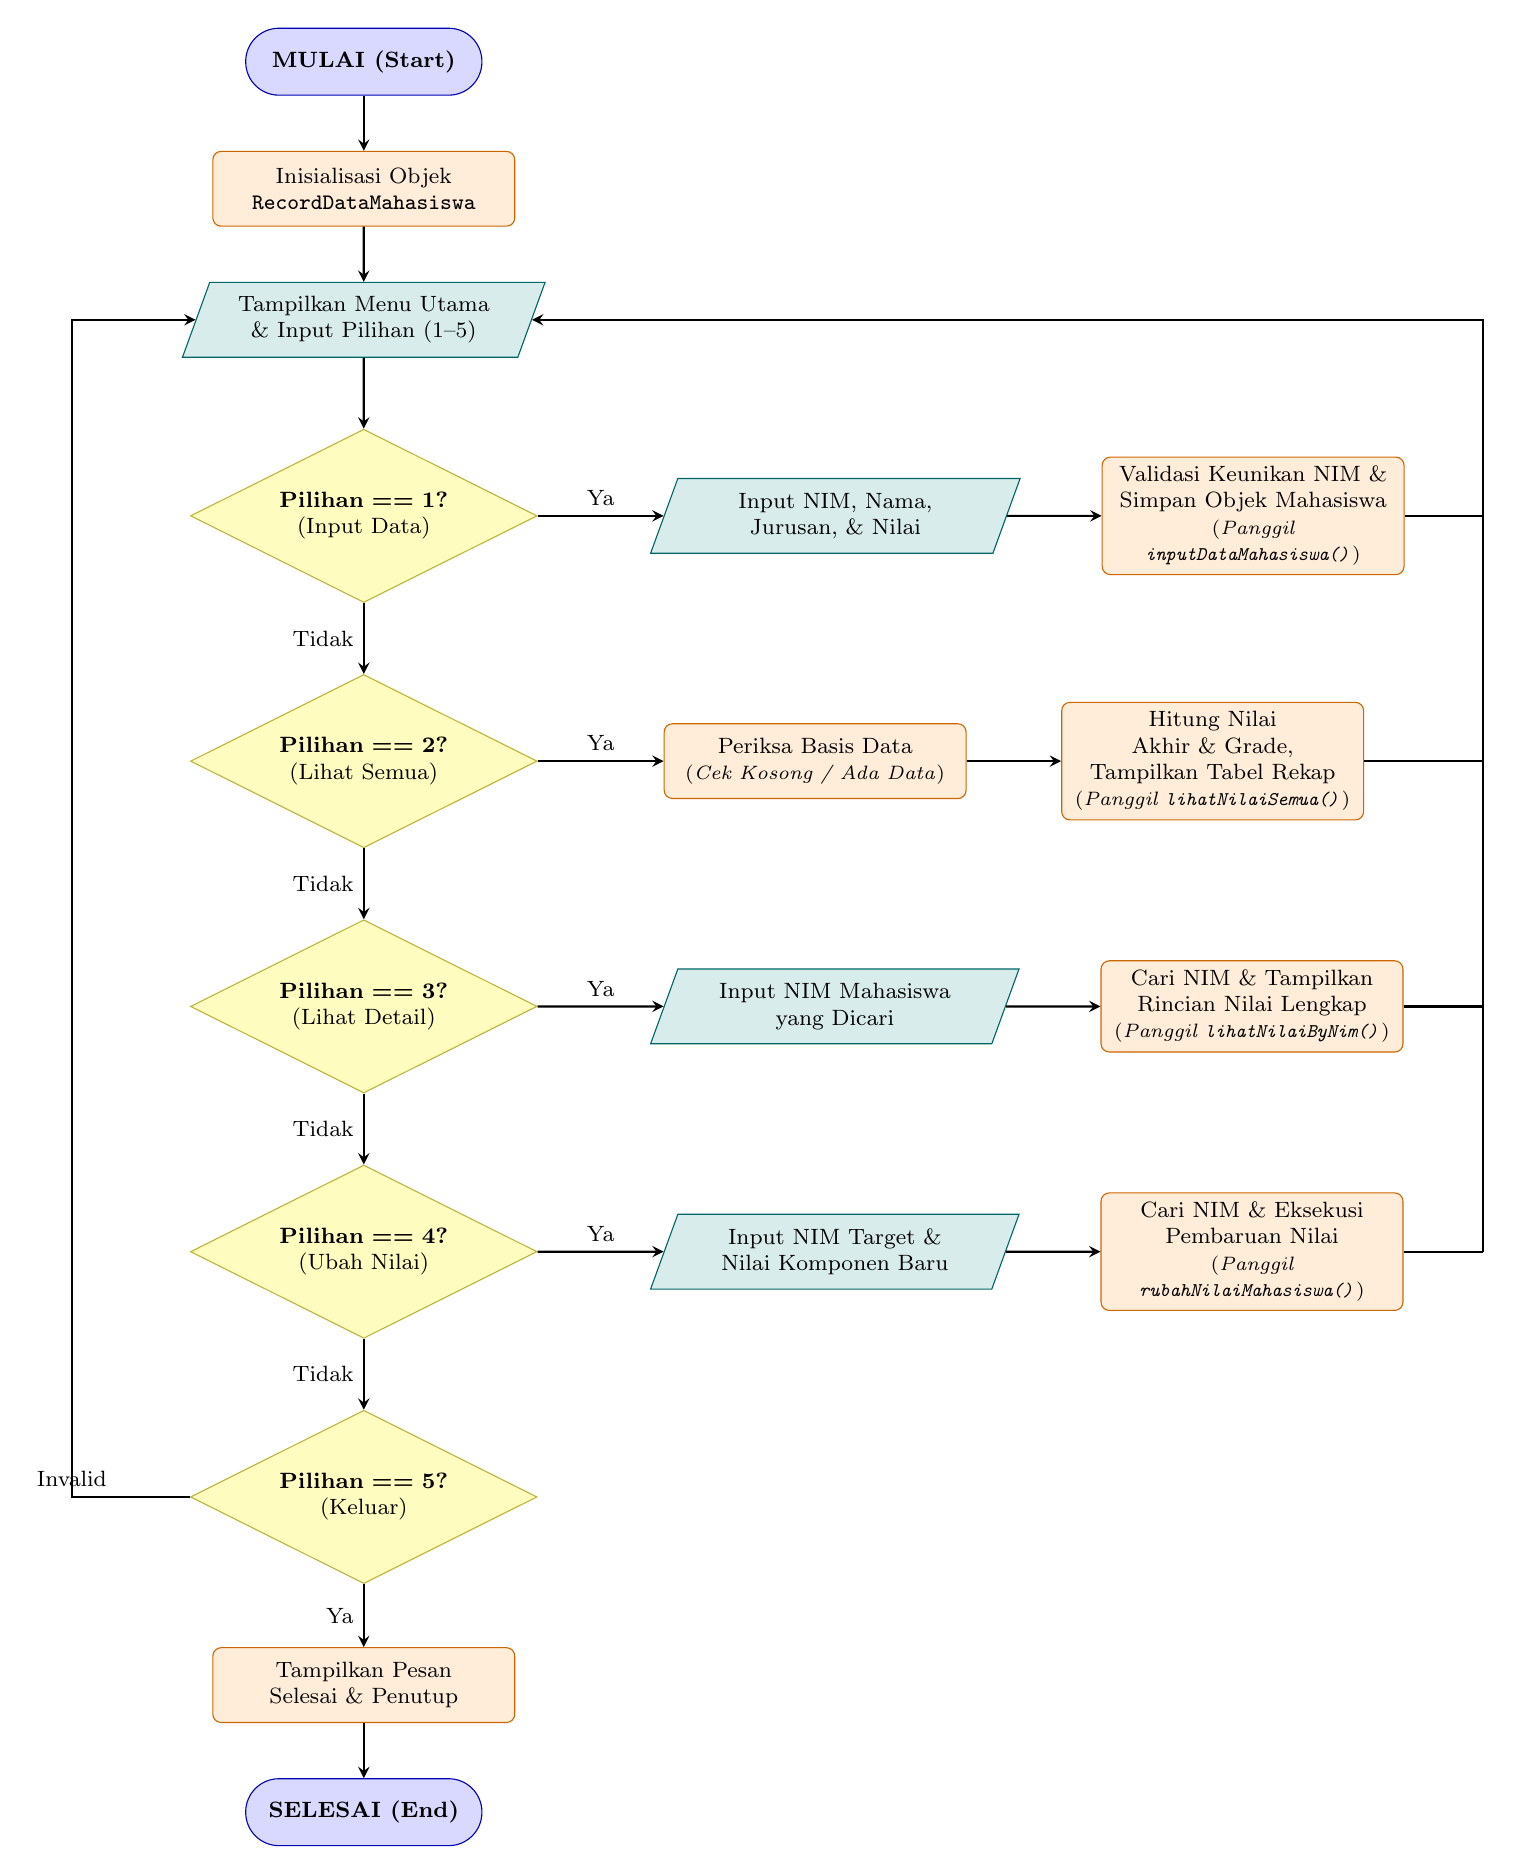
\begin{tikzpicture}[
    node distance=1.3cm,
    auto,
    startstop/.style = {rectangle, rounded corners=12pt, minimum width=3.0cm, minimum height=0.85cm, text centered, draw=blue!70!black, fill=blue!15, font=\bfseries\footnotesize},
    process/.style   = {rectangle, rounded corners=3pt, minimum width=3.5cm, minimum height=0.95cm, text centered, draw=orange!80!black, fill=orange!15, text width=3.6cm, font=\footnotesize},
    decision/.style  = {diamond, aspect=2, minimum width=2.8cm, minimum height=0.85cm, text centered, draw=yellow!70!black, fill=yellow!25, text width=2.5cm, font=\footnotesize},
    io/.style        = {trapezium, trapezium left angle=70, trapezium right angle=110, minimum width=3.2cm, minimum height=0.95cm, text centered, draw=teal!80!black, fill=teal!15, text width=3.2cm, font=\footnotesize},
    arrow/.style     = {thick, ->, >=stealth}
]

    % --- Tulang Punggung Utama (Spine Vertikal) ---
    \node (start) [startstop] {MULAI (Start)};
    \node (init)  [process, below=0.7cm of start] {Inisialisasi Objek\\ \texttt{RecordDataMahasiswa}};
    \node (menu)  [io, below=0.7cm of init] {Tampilkan Menu Utama\\ \& Input Pilihan (1--5)};
    
    % Decision Pilihan Menu
    \node (dec1)  [decision, below=0.9cm of menu] {\textbf{Pilihan == 1?}\\(Input Data)};
    \node (dec2)  [decision, below=0.9cm of dec1] {\textbf{Pilihan == 2?}\\(Lihat Semua)};
    \node (dec3)  [decision, below=0.9cm of dec2] {\textbf{Pilihan == 3?}\\(Lihat Detail)};
    \node (dec4)  [decision, below=0.9cm of dec3] {\textbf{Pilihan == 4?}\\(Ubah Nilai)};
    \node (dec5)  [decision, below=0.9cm of dec4] {\textbf{Pilihan == 5?}\\(Keluar)};
    
    % Exit & Selesai
    \node (exit)  [process, below=0.8cm of dec5] {Tampilkan Pesan\\ Selesai \& Penutup};
    \node (stop)  [startstop, below=0.7cm of exit] {SELESAI (End)};

    % --- Cabang Menu 1: Input Data ---
    \node (p1_in)   [io, right=1.6cm of dec1] {Input NIM, Nama,\\ Jurusan, \& Nilai};
    \node (p1_proc) [process, right=1.2cm of p1_in] {Validasi Keunikan NIM \&\\ Simpan Objek Mahasiswa\\ \scriptsize(\textit{Panggil \texttt{inputDataMahasiswa()}})};

    % --- Cabang Menu 2: Lihat Semua ---
    \node (p2_in)   [process, right=1.6cm of dec2] {Periksa Basis Data\\ \scriptsize(\textit{Cek Kosong / Ada Data})};
    \node (p2_proc) [process, right=1.2cm of p2_in] {Hitung Nilai Akhir \& Grade,\\ Tampilkan Tabel Rekap\\ \scriptsize(\textit{Panggil \texttt{lihatNilaiSemua()}})};

    % --- Cabang Menu 3: Lihat Detail ---
    \node (p3_in)   [io, right=1.6cm of dec3] {Input NIM Mahasiswa\\ yang Dicari};
    \node (p3_proc) [process, right=1.2cm of p3_in] {Cari NIM \& Tampilkan\\ Rincian Nilai Lengkap\\ \scriptsize(\textit{Panggil \texttt{lihatNilaiByNim()}})};

    % --- Cabang Menu 4: Ubah Nilai ---
    \node (p4_in)   [io, right=1.6cm of dec4] {Input NIM Target \&\\ Nilai Komponen Baru};
    \node (p4_proc) [process, right=1.2cm of p4_in] {Cari NIM \& Eksekusi\\ Pembaruan Nilai\\ \scriptsize(\textit{Panggil \texttt{rubahNilaiMahasiswa()}})};

    % --- Titik Jalur Bus Kembali ke Menu ---
    \coordinate (bus) at ([xshift=1.0cm]p1_proc.east);

    % --- Garis Spine Vertikal ---
    \draw [arrow] (start) -- (init);
    \draw [arrow] (init) -- (menu);
    \draw [arrow] (menu) -- (dec1);
    \draw [arrow] (dec1) -- node[left, font=\footnotesize] {Tidak} (dec2);
    \draw [arrow] (dec2) -- node[left, font=\footnotesize] {Tidak} (dec3);
    \draw [arrow] (dec3) -- node[left, font=\footnotesize] {Tidak} (dec4);
    \draw [arrow] (dec4) -- node[left, font=\footnotesize] {Tidak} (dec5);
    \draw [arrow] (dec5) -- node[left, font=\footnotesize] {Ya} (exit);
    \draw [arrow] (exit) -- (stop);

    % --- Garis Cabang Menu Horizontal ---
    % Menu 1
    \draw [arrow] (dec1) -- node[above, font=\footnotesize] {Ya} (p1_in);
    \draw [arrow] (p1_in) -- (p1_proc);
    \draw [thick] (p1_proc.east) -- (bus |- p1_proc.east);

    % Menu 2
    \draw [arrow] (dec2) -- node[above, font=\footnotesize] {Ya} (p2_in);
    \draw [arrow] (p2_in) -- (p2_proc);
    \draw [thick] (p2_proc.east) -- (bus |- p2_proc.east);

    % Menu 3
    \draw [arrow] (dec3) -- node[above, font=\footnotesize] {Ya} (p3_in);
    \draw [arrow] (p3_in) -- (p3_proc);
    \draw [thick] (p3_proc.east) -- (bus |- p3_proc.east);

    % Menu 4
    \draw [arrow] (dec4) -- node[above, font=\footnotesize] {Ya} (p4_in);
    \draw [arrow] (p4_in) -- (p4_proc);
    \draw [thick] (p4_proc.east) -- (bus |- p4_proc.east);

    % Jalur Bus Tunggal Kembali ke Menu Utama
    \draw [arrow] (bus |- p4_proc.east) -- (bus |- menu.east) -- (menu.east);

    % Jalur Input Tidak Valid (Sisi Kiri)
    \draw [arrow] (dec5.west) -- ++(-1.5cm,0) node[above, font=\footnotesize] {Invalid} |- (menu.west);

\end{tikzpicture}
\end{document}
